\documentclass[UTF8]{ctexart}

\usepackage{subfiles}  

%下面的语句, 引入你的头部设置文件
\usepackage{C:/phpStorm_proj/02_myself_ID_EGO/+100_latex_all_math_sel/myPreamble} 
%必须是绝对路径,才能让各个tex在单独编译时使用到

\title{文件名}


%---------------------------------


\begin{document}
	\tableofcontents % 生成目录
	\date{} % 若不写这句, 则默认也会渲染出日期, 所以我们要手动赋空值
	\maketitle  %这行代码, 让你前面的 title, author, date生效
	



\part{贝叶斯公式 Bayes' theorem : \\ $ 
		P\left( A_k|B \right) =\dfrac{P\left( A_k \right) \cdot P\left( B|A_k \right)}{\sum_{i=1}^n{\text{[}}P\left( A_i \right) \cdot P\left( B|A_i \right) \text{]}}=\dfrac{P\left( A_kB \right)}{P\left( B \right)}
		$}




\section{先验概率 (从经验来推后果) \& 后验概率(更新迭代经验)}

\begin{tabular}{|p{0.6\textwidth}|p{0.4\textwidth}|}
	\hline
	先验概率 :	是指根据以往经验和分析得到的概率,它往往作为``由因求果"问题中的``因"出现.  
	&   
	``先验概率"的计算比较简单,没有使用``贝叶斯公式". \\
	\hline
	后验概率: 是基于新的信息,修正原来的``先验概率"后, 所获得的更接近实际情况的概率估计.	
	& ``后验概率''的计算,要使用``贝叶斯公式".
	\\
	\hline
\end{tabular} 
\vspace{1em} 



\section{贝叶斯公式: 从``果", 来推是``某因"的可能性大小}

根据新信息, 不断调整对一个随机事件发生概率的判断, 这就是``贝叶斯推理"。 即反复迭代, 不断逼近真相 (即人工智能的原理). \\

通常, ``事件A, 在事件B(发生)的条件下的概率",与``事件B, 在事件A的条件下的概率", 是不一样的. 然而, 这两者是有确定的关系, ``贝叶斯法则"就是对这种关系的陈述。 \\

推导1 : \\
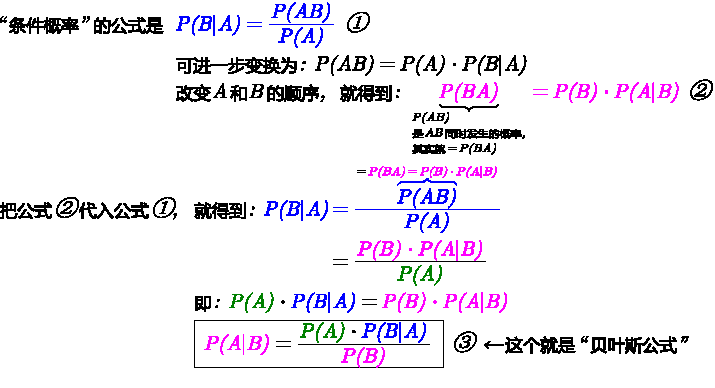
\includegraphics[width=0.9\textwidth]{/0101.pdf} \\

上面``贝叶斯公式"的意思就是说: ``在现象B出现的条件下, 事件A发生的概率" (即 P(A|B)), 就等于``事件A发生的概率 (即 P(A))", 乘以 ``事件A发生条件下, 事件B出现的概率" (即 P(B|A)), 再除以``事件B出现的概率" (即 P(B)). \\



推导2 : \\
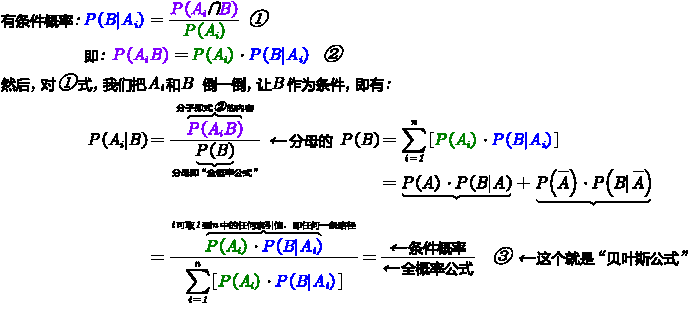
\includegraphics[width=1\textwidth]{/0107.pdf} \\




推导3 : \\
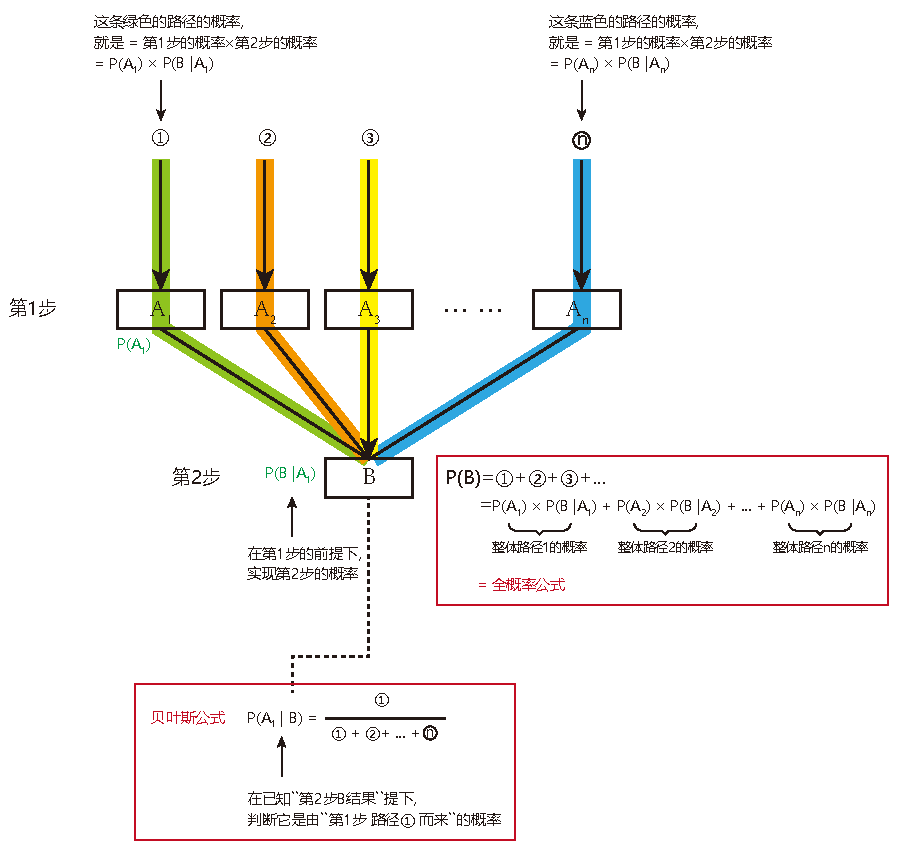
\includegraphics[width=1\textwidth]{/0102.pdf} \\

→ 到第一步的, 其实就是``贝叶斯公式". 即 已知第二步的结果B, 我们来倒推推测它到底是从哪条路径走过来的 (即在第一步中是从哪个路口过来的). 比如, 如果从第$ A_1$ 节点过来, 那么其概率就是:$
P\left( A_1|B \right) =\dfrac{\text{路径1的概率}}{\text{路径1的概率}+\text{路径2的概率}+..+\text{路径}n\text{的概率}}
$ \\
即: \\
$
P\left( A_i|B \right) =\dfrac{P(A_i)\cdot P(B|A_i)}{\sum_{j=1}^n{\left[ P(A_j)\cdot P(B|A_j) \right]}}=\dfrac{\overset{\text{第}i\text{条路径的概率}}{\overbrace{P(A_i)\cdot P(B|A_i)}}}{\underset{\text{分母上是把所有的路径概率,都加起来}=P(B)=\text{全概率公式}}{\underbrace{P(A_1)\cdot P(B|A_1)+...+P(A_n)\cdot P(B|A_n)}}}
$ \\

→ 到第二步的, 其实就是``全概率公式", 即: \\
$
P(B)=\underset{\text{整条路径1的概率}}{\underbrace{P(A_1)\cdot P(B|A_1)}}+\underset{\text{整条路径2的概率}}{\underbrace{P(A_2)\cdot P(B|A_2)}+}...\underset{\text{整条路径}n\text{的概率}}{\underbrace{+P(A_n)\cdot P(B|A_n)}}
$ \\
~\\



宋浩的上课 : \\
有事件 $A_1, A_2, ... A_n$ 组成``完备事件组" (它们作为``原因事件"), $P(A_i) > 0$ \\
有一个事件B (作为``结果事件"), $P(B) > 0$ \\

则: 从B结果, 来倒推推断``它是由第$A_k$个原因造成的"的可能性占多大的概率, 就由这个公式(贝叶斯公式)给出: \\
\begin{align*}  % 支持每行编号. 若不需要编号, 就用 align*环境
	P(\text{原因}A_k\ |\text{结果}B)\\
&=\frac{P(\text{原因}A_k\ \cap \ \text{结果}B)}{P(\text{结果}B)}\\
&=\frac{P\left( \text{原因}A_k \right) \cdot P\left( \text{结果}B\ |\text{原因}A_k \right)}{\sum_{i=1}^n{\left[ P\left( \text{原因}A_i \right) \cdot P\left( \text{结果}B\ |\text{原因}A_i \right) \right]}}\\
&=\frac{A_k\text{这个人,他的责任量}}{\text{所有相关的人}(\text{所有的}A),\text{责任加起来的总和量}} 
\end{align*}
\\




\begin{myEnvSample}
得某病 ← 事件A \\
医院检查出有病 ← 事件B \\
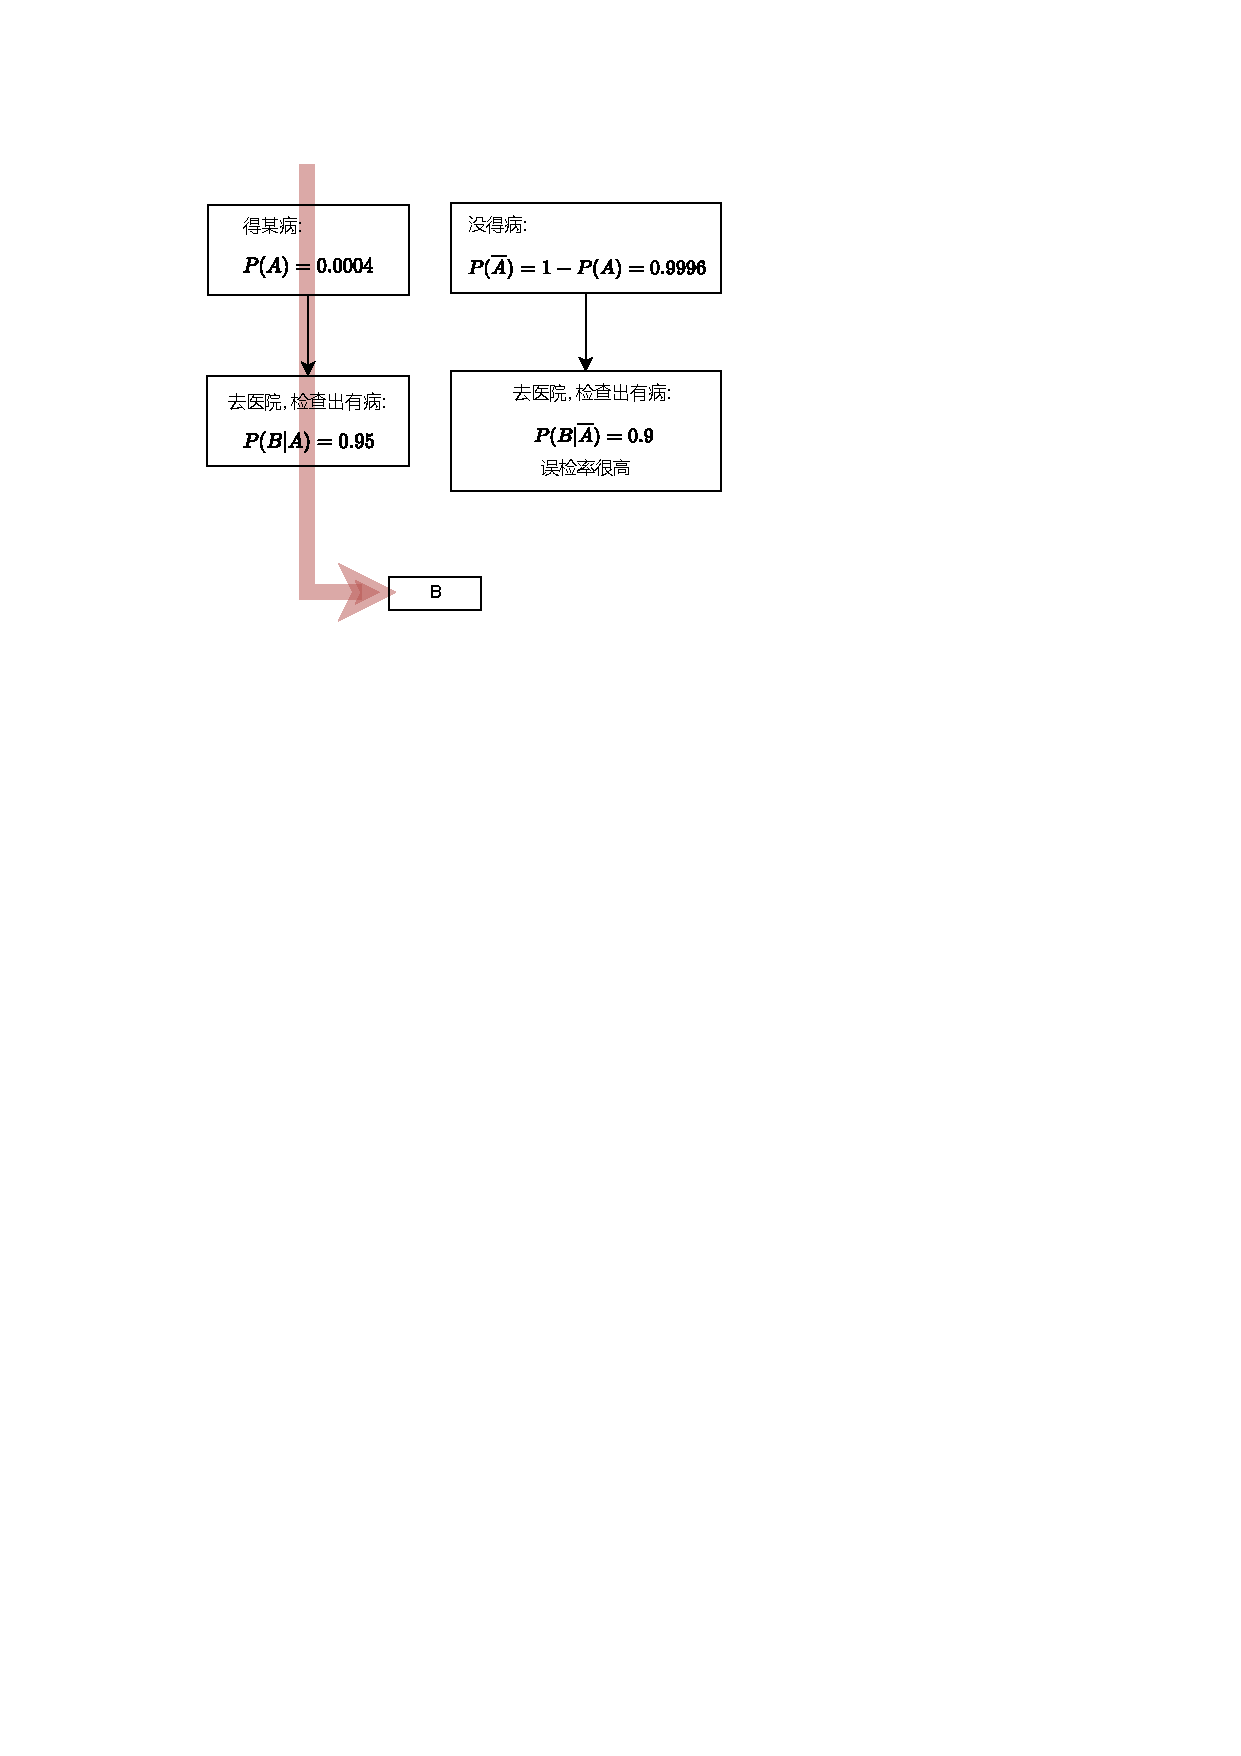
\includegraphics[width=0.6\textwidth]{/0108.pdf}

在某人检测出有病(B)的前提下, 问``其是真实患病(A)"的概率是多少? (即走的是上面红色路径的概率). 即求: $P(A|B) = ?$ 


\begin{align*}  % 支持每行编号. 若不需要编号, 就用 align*环境
	P(A|B)&=\frac{P(AB)}{P(B)}\\
&=\text{或用贝叶斯公式}\frac{P(A_k)\cdot P(B|A_k)}{\sum_{i=1}^n{\left[ P(A_i)\cdot P(B|A_i) \right]}}\\
&=\frac{P(A)\cdot P(B|A)}{P(A)\cdot P(B|A)+P(\overline{A})\cdot P(B|\overline{A})}\\
&=\frac{0.0004\cdot 0.95}{\left( 0.0004\cdot 0.95 \right) +\left( 0.9996\cdot 0.9 \right)}=0.000422213
\end{align*}
\end{myEnvSample}

所以, 你可以看出: \\
- 全概率公式, 是从``原因"来推``结果的可能性是多少". \\
- 贝叶斯公式, 是从``结果"来倒推其``是从哪一种原因得来的"的可能性. 即 $P(\text{原因}_i\ |\text{结果})$ \\





\begin{myEnvSample}
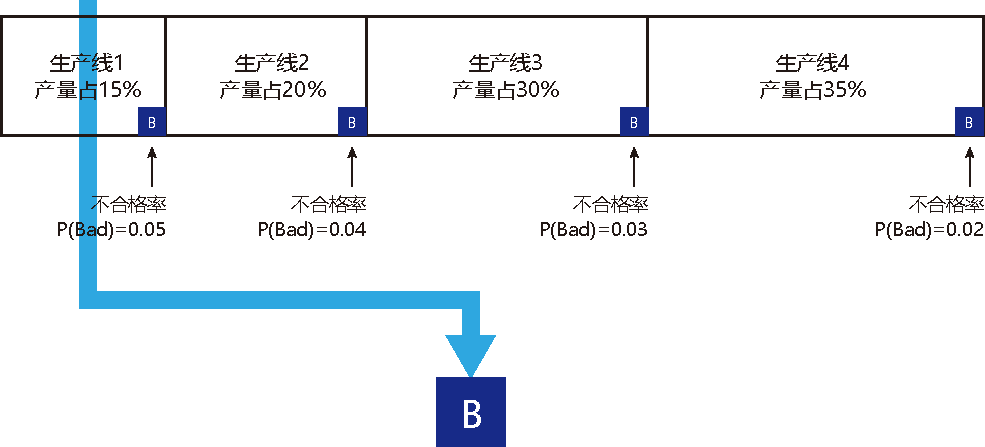
\includegraphics[width=1\textwidth]{/0109.pdf} \\

一个工厂, 有4条生产线, 情况如下: \\
	\begin{tabular}{lllll}
		\hline
		& 生产线1 & 生产线2 & 生产线3 & 生产线4 \\
		\hline
		产量   & 15\% & 20\% & 30\% & 35\% \\
		\hline
		不合格率 & 0.05 & 0.04 & 0.03 & 0.02  \\
		\hline
	\end{tabular} \\

我们设 : \\
- $A_1$ : 代表生产线1的产品 \\
- $A_2$ : 代表生产线2的产品 \\
- $A_3$ : 代表生产线3的产品 \\
- $A_4$ : 代表生产线4的产品 \\
- B (bad) : 代表不合格品. \\

则, 这个工厂的总的不合格率 : 
\begin{align*}  % 支持每行编号. 若不需要编号, 就用 align*环境
P(B)
&=\overset{\text{即}“\text{全概率公式}”}{\overbrace{\underset{\text{第1条生产线的产量占比,乘以第1条生产线的不合格率}}{\underbrace{P(A_1)\cdot P(B|A_1)}}+...+P(A_4)\cdot P(B|A_4)}}\\
&=\left( 0.15\cdot 0.05 \right) +\left( 0.2\cdot 0.04 \right) +\left( 0.3\cdot 0.03 \right) +\left( 0.35\cdot 0.02 \right) =0.0315
\end{align*}

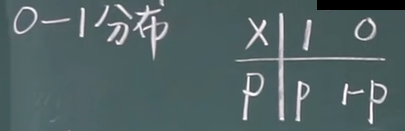
\includegraphics[width=0.75\textwidth]{/0110.png}

现在问: 在发生了B结果的前提下, 它是由 $A_1$ 原因(路径)引起的可能性, 是多少? ← 这就是要用``贝叶斯公式"了. 从``结果",来问``某原因"导致的可能性是多少. \\
$
P(A_1|B)=\dfrac{P\left( A_1B \right)}{P\left( B \right)}=\dfrac{\overset{A_1\text{生产线产量占}0.15}{\overbrace{P\left( A_1 \right) }}\cdot \overset{A_1\text{生产线的不合格率}=0.05}{\overbrace{P(B|A_1)}}}{\underset{\text{这个工厂总的不合格率}=0.0315}{\underbrace{P\left( B \right) }}}=\dfrac{0.15\cdot 0.05}{0.0315}=0.238095
$ \\

同理, 其他原因(其他生产线带来的次品)的可能性是: \\
$P(A_2|B)=\dfrac{P\left( A_2B \right)}{P\left( B \right)}=\dfrac{P\left( A_2 \right) \cdot P(B|A_2)}{P\left( B \right)}=\frac{0.2\cdot 0.04}{0.0315}=0.253968$ \\
$P(A_3|B)=\dfrac{P\left( A_3B \right)}{P\left( B \right)}=\dfrac{P\left( A_3 \right) \cdot P(B|A_3)}{P\left( B \right)}=\frac{0.3\cdot 0.03}{0.0315}=0.285714 $ \\
$P(A_4|B)=\dfrac{P\left( A_4B \right)}{P\left( B \right)}=\dfrac{P\left( A_4 \right) \cdot P(B|A_4)}{P\left( B \right)}=\frac{0.35\cdot 0.02}{0.0315}=0.222222 $ \\

所以, 是第3条生产线造成的原因的可能性最大, 因为其概率值最高.
\end{myEnvSample} 
\vspace{1em} 




\begin{myEnvSample}
某病, 发病率是 0.0004. 有种检测方法, 但存在误诊情况. \\
我们先设定事件: \\
- 事件A: 表示某人真有病,即阳性 \\
- 事件 $\overline{A}$: 表示某人无病, 阴性 
- 事件B : 表示检测认为该人阳性. \\

该检测方法, 准确度如下: \\
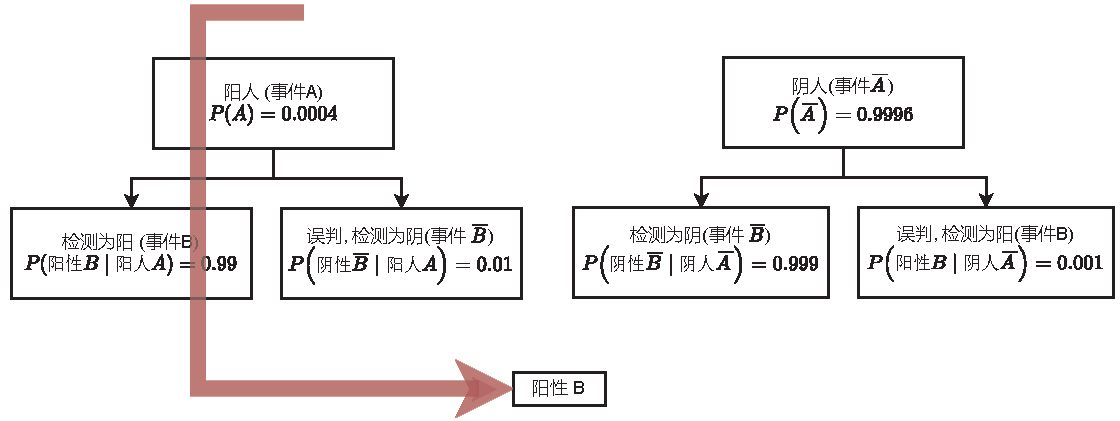
\includegraphics[width=1\textwidth]{/0111.pdf} \\

问: 一个人被检测为``阳", 那么他真的是``得病"的概率是? 即问: $P(\text{阳人}A \ |\text{阳性}B=?)$ 

\begin{align*}  % 支持每行编号. 若不需要编号, 就用 align*环境
	P(A|B) &=\frac{\overset{P(\text{前后})=P(\text{前})\cdot P(\text{后|前})}{\overbrace{P\left( AB \right) }}}{\underset{\text{任何一个人被检测为阳的概率}}{\underbrace{P\left( B \right) }}}=\frac{P\left( A \right) \cdot P\left( B|A \right)}{P\left( B \right)}\\
&=\frac{\overset{=0.0004}{\overbrace{P\left( A \right) }}\cdot \overset{=0.99}{\overbrace{P\left( B|A \right) }}}{\underset{\text{无误诊,将患者}(A)\text{确认为阳性}(B)}{\underbrace{P\left( A \right) \cdot P\left( B|A \right) }}+\underset{\text{有误诊,将阴人}(\overline{A})\text{误诊为阳性}}{\underbrace{\overset{=0.9996}{\overbrace{P\left( \overline{A} \right) }}\cdot \overset{=0.001}{\overbrace{P\left( B|\overline{A} \right) }}}}}\\
&=\frac{0.0004\cdot 0.99}{0.0004\cdot 0.99+0.9996\cdot 0.001}=0.283749
\end{align*}


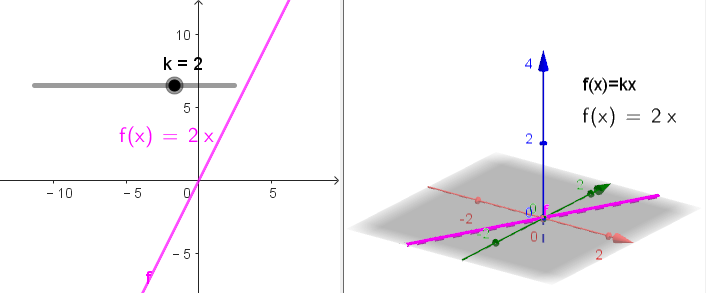
\includegraphics[width=0.3\textwidth]{/0112.png}

\end{myEnvSample}
\vspace{1em} 



概率告诉我们: 要相信长期中的期望.$0.99^{365}=0.025518$, 而 $ 1.01^{365}=37.7834$.   \\
篮球领域有一句名言——``训练时,用正确姿势投丢的球, 比用错误姿势投进的球, 更有价值." \\
站在当下,未来任何事都只是一个概率. \textbf{所谓坚持,所谓努力,其实就是寻找一个大概率成功的方向, 然后相信系统, 相信长期主义.} 当然,你得坚持活着.等到长期的到来.  \\

但行为经济学家发现,人们在决策过程中, 往往并不遵循``贝叶斯规律",而是给予最近发生的事件和最新的经验, 以更多的权重值,更看重近期的事件。面对复杂问题,人们往往会走捷径,依据可能性, 而非概率来做决策. 这种对经典模型的系统性偏离, 称为``偏差". 因此, 投资者在决策判断时, 并非绝对理性.  \\
但长期以来,由于缺乏有力的``能结合人类决策中的理性和感性因素"的替代工具, 经济学家不得不在分析中坚持``贝叶斯法则".



	
	
	
\end{document}